%% LyX 2.1.3 created this file.  For more info, see http://www.lyx.org/.
%% Do not edit unless you really know what you are doing.
\documentclass[english]{article}
\usepackage[T1]{fontenc}
\usepackage[latin9]{inputenc}
\usepackage{graphicx}
\usepackage{babel}
\usepackage{listings}
\renewcommand{\lstlistingname}{Listing}

\begin{document}

\title{A JIT-Less Type-Mapped Dynamic-ISA Virtual Machine for Many-Instance
Applications}

\maketitle
\rule[0.5ex]{1\columnwidth}{2pt}

\begin{figure}[tph]
 \centerline{ \includegraphics[scale=0.5]{/home/stevetest/Documents/University/Treatise/image1.jpeg}}

\end{figure}



\author{ \centerline{ Author: Douglas Bentley}}


\author{ \centerline{ Supervisor: Kevin Naud�}}

\rule[0.5ex]{1\columnwidth}{2pt}


\title{Submitted in partial fulfilment of the degree Baccalaureus Scientiae
(Honores) in Computer Science at the Nelson Mandela Metropolitan University}

\newpage{}


\section*{Acknowledgements}

\newpage{}


\section*{Abstract}

\newpage{}


\section*{Declaration of Own Work}


\paragraph{I declare that the entirety of the work contained in this treatise
is my own, original work, that I am the sole author thereof (save
to the extent explicitly otherwise stated), that reproduction and
publication thereof by Nelson Mandela Metropolitan University will
not infringe any third party rights that I have not previously in
its entirety or in part submitted it for obtaining any qualification. }


\paragraph{Signature:.................. Date:..................}

\newpage{}


\section*{List of Figures}

\newpage{}


\section*{List of Tables}

\newpage{}


\section*{Table of Contents}



\newpage{}


\section{Introduction}


\subsection{Virtual Machines}


\paragraph{To best describe the virtual machine presented in this treatise,
a quick summary of virtual machines follows. The heirarchy of virtual
machines is presented and our virtual machine is situated within it.
Some important virtual machine terminology is introduced.}


\subsubsection{What is a Virtual Machine?}


\paragraph{A \emph{virtual machine} or \emph{VM} is a computer program that
``executes software in the same manner as the machine for which the
software was developed'' \cite[pg9]{JamesE.Smith2005}. This program
is designed to run on some real machine. We call the real machine
that a virtual machine is running on the \emph{host} and the virtual
machine the \emph{guest. }The guest machine provides an execution
environment for software that is designed to run either on the guest
itself or on an actual machine that the virtual machine is emulating.
This means that we can use a virtual machine to run programs that
are incompatable with the host. The virtual machine allows this by
providing a mapping of its state to the state of the host machine
on which it is running \cite[pg4]{JamesE.Smith2005}.}


\subsubsection{The Types of Virtual Machines}


\paragraph{Virtual machines come in two varieties: \emph{process }virtual machines
and \emph{system} virtual machines. }


\paragraph{A process virtual machine is ``capable of supporting an individual
process''\cite[pg9]{JamesE.Smith2005}. This means that the host
runs the guest for as long as a process on the guest machine needs
it. Once the process has completed its execution the guest machine
terminates\cite[pg9]{JamesE.Smith2005}. An example of a process virtual
machine is the Java Virtual Machine or JVM. All java programs run
on the JVM. An instance of the JVM is started when you execute a java
program and killed when its execution is complete.}


\paragraph{A system virtual machine ``provides a complete system environment''
''\cite[pg9]{JamesE.Smith2005}. This means that it can support an
entire operating system on the guest machine and the many processes
that the guest operating system executes. A system virtual machine
will terminate when the system is shut down.}


\subsubsection{The Types of Process Virtual Machines}


\paragraph{Since this treatise outlines a process virtual machine we shall look
at the different types of process virtual machines and ignore the
finer details of system virtual machines. Process virtual machines
can be divided into two categories: \emph{multiprogrammed} \emph{systems}
and \emph{dynamic} \emph{translators}. These are divided along whether
or not the guest machine uses the same instruction set architecture
as the host machine.}


\paragraph{With multiprogramming the guest and host use the same instruction
set. Multiprogramming is supported by most operating systems and allows
a user to run many processes at once by making each process think
it has access to an entire machine instead of only part of a machine
''\cite[pg13]{JamesE.Smith2005}. The OS creates an environment per
process that it terminates when that process ends execution. }


\paragraph{With dynamic translators the instruction set of the host and guest
generally do not match. The virtual machine translates blocks of instructions
meant for the machine it is emulating and translates them into instructions
to be run on the host. Not all code is translated in a dynamic translater.
Only code that is used often enough will be translated as there is
an overhead involved with translating code. The code that is not translated
is interpreted. Interpreted instructions are read, their meaning interpreted
and then executed. This interpretation step must happen each time
a piece of code is executed so code that is executed enough times
will be dynamically translated and cached so later execution is faster.
Dynamically translating in this manner is known as ju\emph{st-in-time
compilation} (JIT compilation).}


\subsubsection{Dynamic vs Statically Typed Programming Languages}


\paragraph{A dynamically typed language is one in which the type information
is associated with values \cite[pg4]{RobertoIerusalimschy}(REF lua
VM intro). An example of a dynamically typed language is javascript
where the var keyword is used for variables and the type is inferred
from the value stored into a variable. A statically typed language
is one in which the type information is associated with the variable.
An example of this is java where variables are declared using keywords
that define their type (\emph{int}, \emph{string} etc).}


\subsubsection{Where Our VM is Situated}


\paragraph{The virtual machine described in this treatise is a process virtual
machine. This process machine will have a new instruction set architecture
and hence will differ from any host machine's ISA. The virtual machine
does not make use of JIT compilation. It is entirely interpreted.
It is also dynamically typed.}


\subsection{A Virtual Machine for Many Instance Applications}


\paragraph{Modern process virtual machines make use of JIT compilers. Both JVM
and .Net make use of a JIT compiler \cite{MSDN,Oracle}. For applications
that run many concurrent instances, like a web server which which
starts up a new process for every client, a virtual machine that makes
use of a JIT compiler defeats the benefits of read-only memory sharing.
Since memory sharing is not possible when using a JIT compiler, if
we wish to take advantage of it a JIT-less virtual machine is needed.
However the JIT compiler compiler is an important feature of a VM
that allows for code given to it at runtime to be compiled into machine
code that can run directly on the host. This compiled code is cached
and allows for future execution to be faster. Sacrificing the JIT
compiler to allow memory sharing presents us with a need to find alternative
ways to let our programs execute quickly.}


\subsubsection{Type-Mapping}


\paragraph{The idea to be explored for a more performant JIT-Less VM for a dynamically
typed language is to make use of a \emph{finite state space}. The
VM has a small number of registers and instructions that it can perform.
For a dynamically typed VM these instructions may be able to take
arguments of different types. For instance an instruction to add may
take two integers or an integer and a float or two floats. The instruction
has to discover the types of the arguments and perform the correct
action. A finite state machine can be used to keep track of the types
of the values in all of the registers. Whenever the type in a register
is changed, the finite state machine makes a state transition that
keeps track of that change. This means we can use the state of the
finite state machine to jump to specialised versions of each instruction
for each combination of inputs. This is an untested approach that
may improve the performance of our VM.}


\subsection{Project Scope}


\paragraph{The project is to develop an implementation of a VM of this nature
and run predetermined benchmarks on it against an alternate version
of it that does not make use of type-mapping. This experiment should
show what benefits the approach has. The VM will only have around
35 instructions and 2 types: integer and pointer. There will be no
compiler or assembler implementation required and the VM will not
be required to perform garbage collection. The VM will also not have
to be robust in how it interacts with the operating system it is running
on nor in how it handles errors.}


\subsection{Risks}


\paragraph{The risks of the project are mainly about its structure and how it
can be criticised. The VM will be running predefined benchmarks. If
it performs those well at the expense of its general usefulness the
project can be criticised. All of these sorts of criticisms can be
mitigated so long as the goal of the project is kept in mind at all
times. Learning as much as possible about how well the idea works
should always take precedence over trying to make results look good.
Whether the VM performs better or not is important knowledge and being
as careful as possible about discovering that accurately is extremely
important.}


\subsection{Overview of Treatise}


\paragraph{To be completed}

\newpage{}


\section{Literature Review, Existing systems and Modern Processors}


\subsection{Modern Processor Architecture}


\paragraph{In order to create an efficient VM, we need first understand how
modern processors work and what some of the bottlenecks for our VM's
execution might be. For example, \emph{threading techniques} (not
to be confused with threads in application programming) are commonly
used in VM design. These take advantage of a feature of modern processors
called the \emph{Branch Target Buffer} or BTB. The BTB exists to aid
a process called \emph{branch prediction}. Branch prediction itself
can only be explained once we know about how modern processors make
use of \emph{pipelining} to increase their throughput. As you can
see, an understanding of modern computer architectures is needed before
we can begin a discussion of VM design.}


\subsubsection{Pipelining}


\paragraph{Pipelining is a process in which a processor's instruction processing
cycle is shared by many consecutive instructions at once. The instruction
processing procedure is split up into smaller stages that can execute
simultaneously. An example of this is the classic RISC pipeline{[}x{]}
which to divides instruction processing into the following steps:
Instruction Fetch (IF), Decode (ID), Execute(EX), Memory Access (MEM)
and Writeback (WB). Each instruction passes a stage and leaves that
part of the processor free to perform that stage on the next instruction.
Thus many instructions (as many as there are stages) can be processed
at once, instead of each instruction having to be completely processed
before the processor is free to move onto the next instruction. The
process is analogous to an asssembly line, where many cars can be
assembled at the same time, each in a different stage of assembly.}

\begin{figure}[tph]
\protect\caption{\protect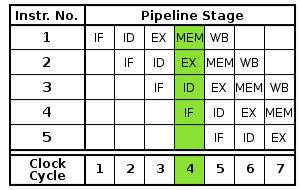
\includegraphics[scale=0.5]{pipeline}}
\end{figure}



\paragraph{In \emph{fig1} we see that the first instruction as currently performing
MEMory access while the second EXecutes and the third is being Decoded.
Up to 5 instructions can be processed simultaneously.}


\paragraph{When pipelining an interesting situation occurs in the case of flow
control instructions. These are instructions that cause execution
to move to some other point in the program. The point at which we
know which instruction comes next (called \emph{branch resolution})
is usually later in the pipeline. Thus the processor cannot queue
up the next instruction as it does not know which instruction will
execute next. Branch prediction is used in modern processors to try
to keep the pipeline as full as possible and not waste time waiting
for this information to be known.}


\subsubsection{Branch Prediction}


\paragraph{Instead of filling up the pipeline with no operation instructions
until we know where to branch, with branch prediction we guess which
branch will be taken and place the instructions from the predicted
branch into the pipeline. When we know where the branch operation
should have taken execution we either throw out our newly pipelined
instructions (this is called \emph{pipeline flushing}) if the prediction
was incorrect or continue execution if it was correct. The more stages
the pipeline has before branch resolution, the more of a performance
benefit correct predictions become for programs with many control
flow instructions. A Virtual Machine is such a program. This is because
a VM must branch to the correct code for each instruction it executes.
Writing code that allows for increased branch prediction accuracy
is thus very important for VM efficiency. }


\paragraph{Predicting a branch means we must predict if that branch is taken
or not and what the target of that branch is if it is taken. Modern
processors have a Branch Target Buffer where the target adresses of
previously taken branches are cached. So upon arrival at a branch
that has been previously taken, we guess if it will be taken and if
it is we begin speculatively executing from the address stored in
the BTB.}


\subsubsection{Cache}


\paragraph{Modern processors make use of different levels of cache to allow
for faster memory access. Ideally we would like to have an infinite
amount of memory with no time cost for accessing it. The reality is
that the larger memory is, the slower it becomes to access it {[}???{]}.
In order to get closer to the ideal modern processors make use of
cache. It takes around 100 cycles for Intel's Intel i7-4770 (Haswell)
architecture to access memory. Cache allows us get get closer to the
ideal case by keeping commonly accessed memory closer to the CPU in
levels of increasingly smaller, faster and more expensive (to manufacture)
memory. The Haswell has 32KB of L1 data cache and 32KB of L1 code
cache. These are located on the CPU itself {[}x{]} and can be accessed
in around 4 cycles{[}x{]}. It also has 256KB of L2 cache and 8 MB
of L3 cache. Caching works on the principal of locality of access.
If you access memory in more or less the same area a lot, that acess
is much faster than if you hop around from place to place. We should
try to take advantage of cache in our VM's design.}


\subsection{Traditional Implementation of High Level VMs}


\subsubsection{Dispatch and Threading}


\paragraph{Dispatch is the process of fetching, decoding and starting the next
instruction to be run by a virtual machine {[}x{]}.}


\paragraph{The simplest way to implement a virtual machine is to make use of
a switch statement in a loop. This is called switch dispatch. Here
is a simplified version to illustrate:}

\begin{lstlisting}
typedef enum { add /* ... */ } Inst; 

void engine() 
{ 
	static Inst program[] = { add /* ... */ }; 
	Inst *ip = program; 
	int *sp; 

	for (;;) 
		switch (*ip++) 
		{ 
		case add: 
			sp[1]=sp[0]+sp[1]; 
			sp++; 
		break; 
		/* ... */ 
	}
} 
\end{lstlisting}



\paragraph{This approach is problematic because the switch statement means that
there is only ever a single entry in the Branch Target Buffer used
for dispatch . This means that the number of mispredictions will be
large as the target of the branch will change for each new instruction
we branch to. This problem may even be magnified by the fact that
this specific VM implementation has far more instructions than usual
as it requires several specialised versions of every instruction.}


\paragraph{A faster alternative to switch dispatch is direct threading\cite{Ertl}.
The name threading comes from the idea of the execution threading
its way from one instruction to the next {[}x{]}. In direct threading
the program is stored as a list of addresses of instructions and the
code for each instruction includes a dispatch portion which jumps
to the address of the next instruction to be executed.}

\begin{lstlisting}
typedef void *Inst; 

void engine() 
{ 
	static Inst program[] = { &&add /* ... */ }; 
	Inst *ip = program; 
	int *sp; 
	
	goto *ip++; /* dispatch first VM inst. */ 

add: 
	sp[1]=sp[0]+sp[1]; 
	sp++; 
	goto *ip++; /* dispatch next VM inst. */ 

}
\end{lstlisting}



\paragraph{Another method is indirect threading. In indirect threading we keep
a lookup table of the addresses of code for each instruction and have
each instruction jump to the next by reading the opcode of the next
instruction from the program, looking up the address of the code for
that instruction in the table and then jumping to that instruction.}

\begin{lstlisting}
typedef void *Inst; 

void engine() 
{ 
	static Inst lookup[] = { &&add, &&sub /*...*/ }
	static int program[] = { 0, /* ... */ }; 
	int *ip = program; 
	int *sp; 
	
	goto *ip++; /* dispatch first VM inst. */ 

add: 
	sp[1]=sp[0]+sp[1]; 
	sp++; 
	goto lookup[*ip++]; /* dispatch next VM inst. */ 
}
\end{lstlisting}



\paragraph{Direct and inderect threading make much better use of the branch
target buffer. Instead of a single entry in the BTB, with direct threading
we have an entry per instruction, so instructions that commonly follow
each other have a better chance of being predicted.}

All code in this section is from or adapted from \cite{M.AntonErtl2003}.


\subsubsection{Registers VS Stacks}


\paragraph{In a stack virtual machine, instructions act on members of the stack.
Arguments and return values for instructions are often implicit and
thus instructions can be smaller. For instance a stack implementation
of a = b + c would first push b and c onto the stack, then call the
add instruction which has no arguments. Add pops b and c off the stack
and pushes b+c back onto the stack. This value is then popped off
the stack and stored.}


\paragraph{For a register machine, a similar piece of code would have values
for b and c in registers and an add instruction is called with a,
b and c as arguments. This instruction would compute b+c and store
it in a regsiter.}


\paragraph{Widely used process virtual machines make use of a stack architecture.
Both the Java Virtual Machine (JVM) and Microsoft's Common Language
Runtime (CLR) make use of stack virtual machines{[}x{]}. }


\subsubsection{JIT Compilation}


\paragraph{Both the JVM and CLR make use of JIT compilation {[}x{]}. JIT compilation
allows for code that is executed often enough to be compiled into
native machine code at runtime. JIT compilation does not preclude
the bytecode of a many-instance application being shared but each
instance of the application is JIT compiling that code. So it is likely
that the same bytecode is being compiled in many different processes
at the same time.}


\subsection{VM Interpreter Reseach}


\paragraph{James R. Bell introduced the concept of threaded code in 1973. The
Fortran IV compiler was written to generate threaded code.\cite{Bell}}


\paragraph{Yuhne Shi\cite{Shi2007} found that a well-implemented register VM
is a more efficient option when speed of execution is more important
than the size of the code to be executed.}


\paragraph{Ertl and Gregg found that in their benchmarks 3.2\%\textendash 13\%
of all executed instructions were indirect branches and that switch
dispatch on an architecture with a BRB resulted in 81\%-98\% branch
prediction misses \cite{M.AntonErtl2003}. They also found that direct
threading resulted in 50\%-63\% branch prediction misses.}


\subsection{Our Implementation}


\subsubsection{Virtual Machine Design Details}


\paragraph{The virtual machine described in this treatise is a register machine.
It has 6 general purpose registers and 3 special purpose registers.
The VM is for a dynamically typed language. Each register stores 'values'
and all instructions act on those values. The type of a value is stored
together with the data for that value. These are implemented in C
as tagged unions. The VM has only two types: integer and pointer. }


\paragraph{The 3 special purpose registers are:}
\begin{enumerate}
\item The program counter (pc), which keeps track of where we are in the
program
\item The frame pointer (fp), which points to the bottom of the latest stack
frame
\item The type state (ts), which keeps track of the current state of types
in the registers
\end{enumerate}

\subsubsection{Type-Mapping}


\paragraph{The virtual machine does not make use of the usual opcode and arguments
arrangment used in register machine interpreters. Usually, the interpreter
reads in some instruction stored as an opcode and the arguments for
that opcode at the same time. In \emph{fig 2} we see a 16 bit instruction
composed of a 4 bit opcode in the high bits, followed by two 6 bit
operands or aguments. The interpreter performs the necessary shifts
and bitmasking to get the values out of the fields.}

\begin{figure}[tph]
\protect\caption{\protect\includegraphics[scale=0.6]{/home/stevetest/opcode}}
\end{figure}



\paragraph{In our VM instructions for programs are stored as opcodes only with
no arguments. That is because we have a version of each instruction
for every combination of registers as inputs. Because we have 6 registers
and a maximum of two arguments per instruction that means that we
can have a maximum of 6\textasciicircum{}2 versions of each instruction.
This saves us the process of extracting arguments at the expense having
to have more versions of the instruction{[}why are we doing it this
way actually?{]}. The opcode implicitly stores the argument information.}


\paragraph{The opcode is not the only information the VM uses to select code,
however. The \emph{ts} register keeps a record of the type of every
register. It is a 6 bit number where each bit tells us the current
type of a register. Thus for every opcode, there are 2\textasciicircum{}6
different states the VM could be in. With this information we know
the arguments and types and can jump to specialised code that acts
on arguments of those types. A good way to think about it is to imagine
it as a 2D lookup table (even though the implementation is 1D). On
the y-axis we have the opcodes for all the versions of the instructions
and on the x-axis we have the current state from 0 to 63. At the intersection
of these we store the address of the code we jump to for that instruction.}


\paragraph{Now since we only have integers and pointers it may, at first glace,
seem pointless to have specialised instructions since most of the
time using pointers in an instruction meant for integers is illegal.
However this method elliminates the type checking involved in instructions
for a dynamic-ISA VM. Normally for each instruction we would have
to check the validity of the arguments first before we can perform
the instruction, but with this method we already know the types and
so we can just jump directly to code for those types or an error if
the arguments are illegal.}


\subsubsection{Indirect Threading}


\paragraph{This VM will make use of indirect threading. Though indirect threading
is slower than direct threading {[}x{]} because it must first complete
the lookup step before it can branch to the next instruction, the
program code used by the VM is intended to be shared by many instances
of the VM. This cannot be achieved with direct threading as the addresses
of each instruction in each instance may be different{[}x{]}. Also
because our dispatch is based on the runtime state of the virtual
machine (the st register) even if addresses were the same between
instnces we can't represent code in terms of those addresses as we
don't know the state information until runtime so we can't choose
which address should be used to replace the opcode. With Indirect
threading's lookup table we can share the code in its opcode form
and perform the correct jumps for each instance of the VM by consulting
the state register and looking up the addresses in the lookup table.}


\paragraph{\newpage{}}

\bibliographystyle{plain}
\bibliography{/home/stevetest/a}

\end{document}
